%!TEX root = ../RASD/main.tex
\newpage
\subsection{Alloy} % (fold)
In this section we provide an Alloy model for the \emph{system-to-be}.\\
The Alloy model includes all major requirements and constrains and checks the consistency of the most important components of the application.

We explicitly chose not to implement the possibility of one \emph{\nameref{def:user}} to to request a taxi for multiple people. This choice is due to the fact that, having relatively large taxis with a relatively large number of available seats, we could have incurred in overflow problems when calculating the sum of the alloy ``Int" primitive.
We believe that this choice is not limiting the model, that would need just one more property to a \emph{signature} and one more \emph{fact} in order to implement that.
\newpage

\subsubsection{Alloy code}
\lstinputlisting[language=alloy]{../alloy/alloymodel.als}



\begin{landscape}
\subsubsection{Alloy world considerations} % (fold)
\label{ssub:alloy-world-considerations}
\begin{figure}[h!t]
\caption{The world generated by the predicate \emph{showGeneral}.}
	\noindent\makebox[\textwidth]{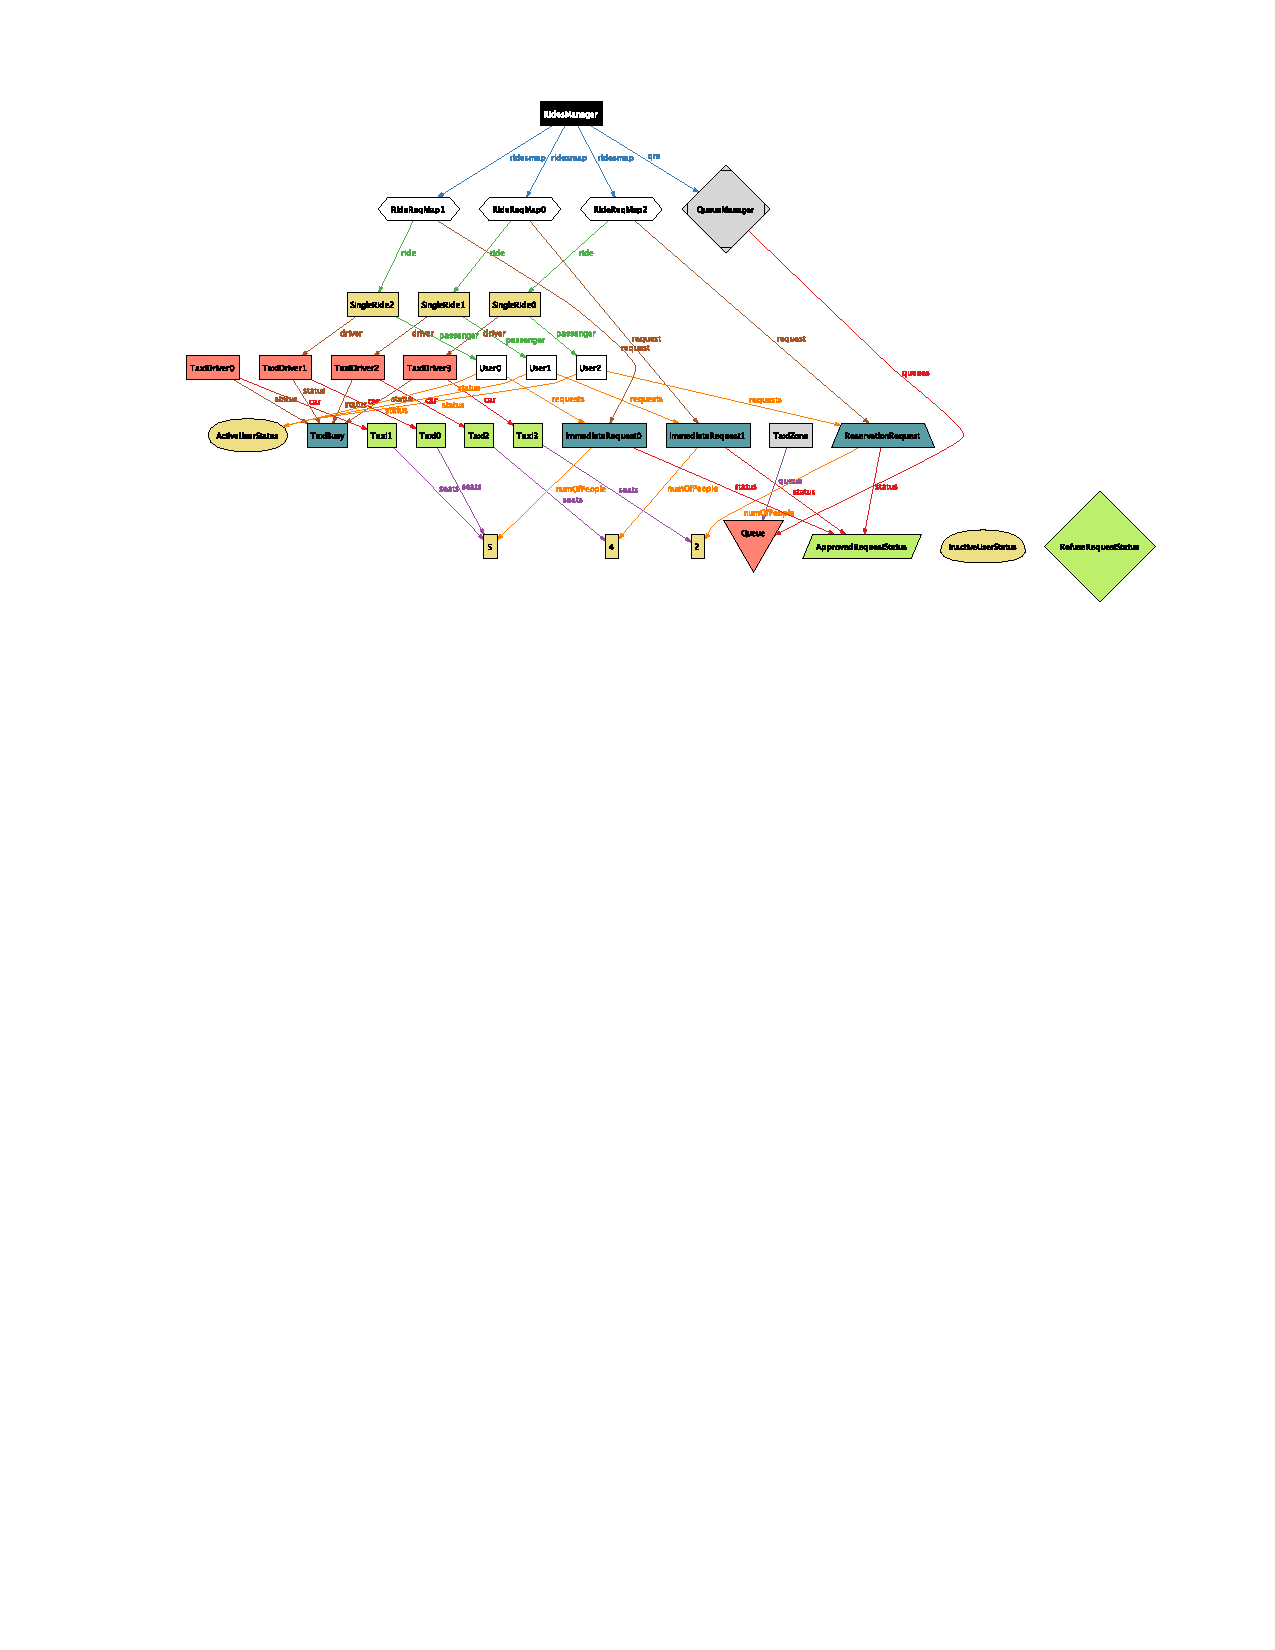
\includegraphics[width=\paperwidth]{alloy/alloyworld}}
\centering
\end{figure}
\end{landscape}

We chose some minimum numbers for the cardinality of the key objects, in order to showcase some of the core relationships that make up the foundations of the modeled world.

We decided to generate two instances of \emph{Ride}, one for each kind, that is one \emph{\nameref{def:single-ride}} and one \emph{\nameref{def:shared-ride}}. The former involves only one \emph{\nameref{def:user}}, while the latter two \emph{\nameref{def:user}s}. 

The number of \emph{\nameref{def:user}s} is enough to have some involved in a ride and others that are inactive.

We also have one more taxi driver than the ones needed for the rides, in order to showcase the queue implementation and the taxi zones.

% subsubsection model-analysis (end)

